\documentclass[a4paper]{article}

\usepackage{graphicx}
\usepackage{float}
\usepackage{hyperref}
\usepackage{enumitem}
\usepackage[utf8]{inputenc}
\usepackage{tocloft}

\setlength\cftbeforesecskip{1pt}
\setlength\cftaftertoctitleskip{2pt}

\setlist[enumerate]{noitemsep}
\setlist[itemize]{noitemsep}

\begin{document}

\title{Performance Report}

\author{\tt more.andres@gmail.com}

\maketitle

\abstract{Report generated using {\tt TBD version 0.0.1}. Please report issues to {\tt more.andres@gmail.com}. Full Log: {\tt mm-full-20130707-090437.log}. Homepage \href{TBD}{http://www.github.com/perf}}

\tableofcontents

\section{Program}

This section provides details about the program being analyzed.
It is used for results reference.

\begin{enumerate}
\item Program: {\tt mm}
\item Source Checksum:\\ {\tt 6ead354fcf0ee8ea3f761e7b6d8ee939}
\item Timestamp: {\tt 20130707-090437}
\item Parameter Range: {\tt 1024-4096}
\item Host: {\tt ubuntu@ubuntu}
\item Distribution: {\tt Ubuntu 12.04.2 LTS}
\item Compiler: {\tt gcc version 4.6.3}
\end{enumerate}

More: \href{TBD}{\tt mm-program-20130707-090437.log}

\section{System Capabilities}

This section provides details about the system being used for the analysis.
It is used as a baseline and for comparison against other configurations.

\subsection{System Configuration}

This  subsection provides details about the bill of materials of the system.

\begin{table}[H]
    \caption{Software/Hardware Configuration}
    \centering
    \begin{tabular}{|l|l|}\hline
      {\bf Component} & {\bf Description} \\ \hline
      Server Board & Intel\textregistered S5000PAL Server Board\\ \hline
      CPU & Intel\textregistered Xeon\textregistered X5355 2.66GHz 8MB L2 \\ \hline
      Ethernet & Intel\textregistered 80003ES2LAN (Copper) (rev 01) \\ \hline
      RAM Memory & 4 GB DDR2 FB 667 MHz \\ \hline
      Distro & Red Hat Enterprise 5.5 (Tikanga) \\ \hline
      Network Driver & Intel\textregistered PRO/1000 1.2.20-NAPI \\ \hline
      Switch & Hewlett Packard HPJ4904A \\ \hline
    \end{tabular}
    \label{table:testbed}
\end{table}

More: \href{TBD}{\tt mm-bom-20130707-090437.log}

\subsection{System Performance Baseline}

This subsection shows reference performance figures from well-known benchmarks.

\begin{table}[H]
\caption{Benchmarks}
  \centering
    \begin{tabular}{|l|l|l|}\hline
      {\bf Benchmark} & {\bf Valor} & {\bf Unidad} \\ \hline
      dgemm & 70141 & mflops \\ \hline
      stream & 5931.6635 & MB/s \\ \hline
      hpl & 0.1217 & tflops \\ \hline
      ping pong BW & 1183.68 & MB/s \\ \hline
      ping pong latency & 4.49 & us \\ \hline
    \end{tabular}
 \label{table:pruebas}
\end{table}

More: \href{TBD}{\tt mm-benchmark-20130707-090437.log}

\section{Workload}

This section provides details about the workload behavior.

\begin{enumerate}
\item Execution time:
\begin{enumerate}
\item problem size: {\tt 4096}
\item geomean: {\tt 5.185585} seconds
\item average: {\tt 5.185638} seconds
\item stddev: {\tt 0.062561}
\item range: {\tt 5.1 - 5.312} seconds
\item repetitions: {\tt 16} times
\item outliers: {\tt None}
\end{enumerate}

\begin{figure}[H]
\label{fig:normal}
\centering
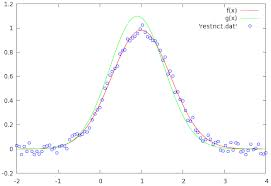
\includegraphics[width=\textwidth]{normal.jpg}
\caption{Results Distribution}
\end{figure}

\end{enumerate}

More: \href{TBD}{\tt mm-workload-20130707-090437.log}

\section{Scalability}

This section provides details about the scaling behavior of the program.

\begin{figure}[H]
\label{fig:normal}
\centering
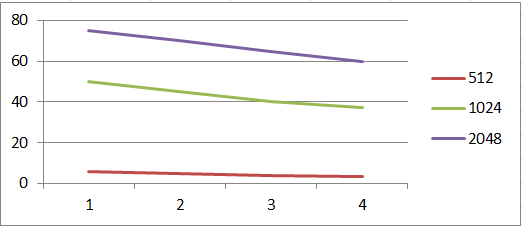
\includegraphics[width=\textwidth]{scaling-time.png}
\caption{Scaling Times}
\end{figure}

\begin{figure}[H]
\label{fig:normal}
\centering
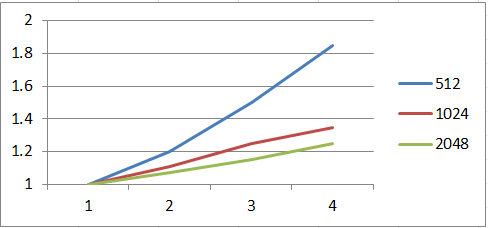
\includegraphics[width=\textwidth]{scaling-ratio.png}
\caption{Scaling Ratio}
\end{figure}

\begin{enumerate}
\item Parallel Fraction: {\tt 80.6\%}
\item Serial: {\tt 19.40\%}
\item Amdalah for 1024 procs: {\tt 5.13 times}
\item Gustafson for 1024 procs: {\tt 825.538 times}
\end{enumerate}

More: \href{TBD}{\tt mm-scaling-20130707-090437.log}

\section{Profile}

This section provides details about the execution profile of the program and the system.

\subsection{Program Profiling}

This subsection provides details about the program execution profile.

\subsubsection{Call Graph}

\begin{verbatim}
92.6% main -> fft -> _fft -> _muldc3
\end{verbatim}

More: \href{TBD}{\tt mm-callgraph-20130707-090437.log}

\subsubsection{Flat Profile}

\begin{verbatim}
77.78% mm.c:27
20.17% mm.c:26
\end{verbatim}

More: \href{TBD}{\tt mm-flatprofile-20130707-090437.log}

Overhead: {\tt 8.1\%}

\subsection{System Profiling}

This subsection provide details about the system execution profile.

\subsubsection{Bottlenecks}

\begin{verbatim}
    for (i = 0; i < SIZE; ++i) {
      for (j = 0; j < SIZE; ++j) {
        for (k = 0; k < SIZE; ++k) {
          c[i][j] += a[i][k] * b[k][j];
0.58 movups (%rax),%xmm0
0.25 add    $0x4,%rax
0.06 shufps $0x0,%xmm0,%xmm0
1.36 mulps  (%rdx),%xmm0
77.20 add    $0x1000,%rdx

          c[i][j] += a[i][k] * b[k][j];
16.94 addps  %xmm0,%xmm1
\end{verbatim}

Overhead: {\tt 15\%}

More: \href{TBD}{\tt mm-bottlenecks-20130707-090437.log}

\subsubsection{System Resources Usage}

\begin{figure}[H]
\label{fig:resources}
\centering
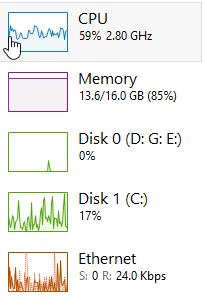
\includegraphics{resources.png}
\caption{Resource Profile}
\end{figure}

More: \href{TBD}{\tt mm-resources-20130707-090437.log}

\section{Low Level}

This section provide details about low level details such as vectorization and performance counters.

\subsection{Vectorization Report}

This subsection provide details about vectorization status of the program loops.

\begin{verbatim}
mm.c:25: LOOP VECTORIZED.
mm.c:13: complicated access pattern.
mm.c:14: LOOP VECTORIZED.
\end{verbatim}

More: \href{TBD}{\tt mm-vectorization-20130707-090437.log}

\subsection{Counters Report}

This subsection provides details about software and hardware counters.

\begin{verbatim}
6 CPU-migrations
3,300 page-faults
1230 cycles
456 stalled-cycles-frontend
789 stalled-cycles-backend
123 branch-misses
\end{verbatim}

More: \href{TBD}{\tt mm-counters-20130707-090437.log}

\end{document}